\chapter{Filtro de Wiener}
\label{chapter:wiener}

Começaremos nossa análise de métodos de identificação com o Filtro de
Wiener~\cite{hayes-1996}. Mais especificamente, usaremos uma versão do modelo que
contempla apenas distorções lineares na estimação: como sua saída é computada por meio
de uma convolução linear entre o filtro calculado e a entrada, definiremos esta como
sendo o sinal original. Assim, o algoritmo será incapaz de introduzir harmônicos na
entrada, e, portanto, seu desempenho no contexto do projeto será limitado. Todavia,
como um método não-linear deve ser capaz de reproduzir linearidades, os resultados
deste capítulo servirão como valores de referência nas análises dos demais métodos.

Desenvolvido por Norbert Wiener durante os anos 1940~\cite{wiener-1949}, o Filtro de
Wiener ganhou notoriedade por sua simplicidade e robustez, sendo um dos primeiros
métodos a adotar uma abordagem estatística em sua modelagem. Ele é caracterizado por
ser um \emph{filtro linear ótimo} para o erro quadrático médio entre o sinal observado
e o estimado. Curiosamente, o pesquisador soviético Andrei Kolmogorov desenvolveu
independentemente as equações do filtro para sinais discretos, publicando seu trabalho
em 1941~\cite{kolmogorov-1941}; por este motivo, o método é algumas vezes chamado de
Filtro de Wiener-Kolmogorov, embora esta seja uma alcunha muito mais rara.

Este capítulo se inicia formulando o problema a ser considerado. Então, o Filtro de
Wiener FIR (de \textit{Finite-length Impulse Response}, ou Resposta ao Impulso de
Comprimento Finito) para sinais discretos será formalmente deduzido e suas equações
serão apresentadas. Em seguida, o algoritmo específico aplicado no trabalho será
explicitado, e seu desempenho será avaliado com uma série de experimentos em sinais de
áudio com distorções lineares e/ou não-lineares.

\section{Formulação do problema}
\label{section:wiener:wiener-model}

O Filtro de Wiener pode ser empregado, dentre outras aplicações, para predição linear,
cancelamento de ruído, ou, como no caso do trabalho em questão, estimação de um sinal
filtrado. Seja qual for o contexto, o cerne do problema é sempre o mesmo: encontrar um
filtro que minimize o erro quadrático médio entre sua saída e um sinal desejado.

Abstraindo a terminologia apresentada no Capítulo~\ref{chapter:intro}, considere o
sinal de referência $d[n]$ e o sinal observado $x[n]$. Supõe-se que ambos são amostras
de sequências aleatórias estacionárias no sentido amplo
(WSS\abbrev{WSS}{\textit{Wide-Sense Stationary}}, de \textit{Wide-Sense
	Stationary})~\cite{peebles-1987}. Nosso objetivo é encontrar o filtro
$W(z)$\symbl{$W(z)$}{Transformada Z do Filtro de Wiener} com resposta ao impulso
$w[n]$\symbl{$w{[n]}$}{Resposta ao impulso do Filtro de Wiener}, tal que a estimativa
dada pela convolução linear entre $x[n]$ e $w[n]$,
\begin{equation}
	\hat{d}[n] = (w * x)[n]\symbl{$*$}{Convolução entre dois sinais},
\end{equation}
minimize o erro quadrático médio entre $d[n]$ e $\hat{d}[n]$,
\begin{equation}
	\xi = E\{|e[n]|^2\} = E\{|d[n] - \hat{d}[n]|^2\},
	\label{eq:wf:square-error}
\end{equation}
onde $E\{\cdot\}$\symbl{$E\{\cdot\}$}{Valor esperado estatístico} é o valor esperado estatístico e $e[n] = d[n] - \hat{d}[n]$\symbl{$e{[n]}$}{Erro entre a saída observada e a estimada} é o erro entre a saída obtida e a referência. Como pressupomos que tanto $x[n]$ quanto $d[n]$ são WSS, $\xi$\symbl{$\xi$}{Erro quadrático médio entre a observação e a estimação} é um valor constante para um dado $W(z)$ e, portanto, independente de $n$. Um diagrama de blocos do problema encontra-se na Figura~\ref{fig:wf:sistem-model}. A elaboração foi feita no domínio discreto; a reformulação para sinais contínuos, porém, é imediata.
\begin{figure}[!ht]
	\centering
	\begin{tikzpicture}[node distance=2cm]
	\node[dspnodeopen,dsp/label=above] (x) {$x[n]$};
	\node[dspfilter, right=of x] (W) {$W(z)$};
	\node[dspadder, right=of W] (sub) {};
	\node[xshift=-0.5cm, yshift=0.25cm] (minus) at (sub) {$-$};
	\node[xshift=-0.25cm, yshift=0.5cm] (plus) at (sub) {$+$};
	\node[dspnodeopen,dsp/label=left, above=of sub, yshift=-0.5cm] (d) {$d[n]$};
	\node[dspnodeopen,dsp/label=above, right=of sub] (e) {$e[n]$};
	\draw[dspconn] (x) -- (W);
	\draw[dspconn] (d) -- (sub);
	\draw[dspconn] (sub) -- (e);
	\draw[dspconn] (W) -- node[midway,above] {$\hat{d}[n]$} (sub);
\end{tikzpicture}
	\caption[Diagrama de blocos do problema para o Filtro de Wiener]{Diagrama de blocos do problema para o Filtro de Wiener.}
	\label{fig:wf:sistem-model}
\end{figure}

No problema originalmente proposto por Wiener, $x[n]$ é a versão corrompida por ruído
aditivo de uma referência $d[n]$. No nosso caso, alguns papéis foram trocados: $x[n]$ é
um sinal não-distorcido, e queremos reproduzir as distorções presentes em $d[n]$; este
sinal, porém, está indisponível, e temos apenas $y[n]$, a observação. Esta diferença
conceitual não afeta a derivação das equações do filtro, e retornaremos à terminologia
do trabalho quando o método específico for proposto.

\section{Filtro de Wiener FIR causal}
\label{section:wiener:fir-filter}

Com o problema bem definido, devemos agora discorrer sobre como solucioná-lo. Note que,
na formulação, não foram especificadas as características do filtro ótimo (além de ele
ser discreto, embora tenha sido mencionado seu equivalente contínuo). Isto não foi por
acaso; é possível desenvolver diferentes soluções para o filtro, dependendo das
restrições impostas: se ele será causal ou não-causal, discreto ou contínuo, e com
resposta ao impulso de duração finita ou não.

Neste trabalho, foi estipulado o uso do Filtro de Wiener FIR discreto e causal, visto
que este é relativamente simples de ser derivado e implementado, além de ser
suficientemente eficaz para uma primeira análise do problema de estimação. Ademais,
como estamos tratando de sinais digitais, é natural a escolha de um filtro discreto.
Suas equações serão agora desenvolvidas.

Para esta derivação, além das suposições apresentadas na
Seção~\ref{section:wiener:wiener-model}, consideraremos também que os sinais $x[n]$ e
$d[n]$ são conjuntamente estacionários no sentido amplo, e que sua correlação cruzada
$R_{xd}[k]$\symbl{$R_{\cdot\cdot}{[k]}$}{Autocorrelação ou correlação cruzada} é
conhecida, além de $R_{xx}[k]$, a autocorrelação de $x[n]$. Pressupõe-se também que
todos os sinais são reais.

Se o filtro projetado tem resposta ao impulso finita e é causal, isto significa que sua
Transformada Z é da forma
\begin{equation}
	W(z) = \sum_{n=0}^{L-1} w[n] z^{-n},
\end{equation}
onde $L$\symbl{$L$}{Tamanho do filtro utilizado} é o comprimento do filtro. Além disso,
\begin{equation}
	\hat{d}[n] = (w * x)[n] = \sum_{m = 0}^{L - 1} w[m] x[n - m].
	\label{eq:wf:dhat-conv}
\end{equation}

É possível reescrever esta última equação na forma de uma operação matricial. Para isso, considere o vetor $\mathbf{w}$, composto pelos coeficientes do filtro,
\begin{equation}
	\mathbf{w} = \begin{bmatrix} w[0] & w[1] & \cdots & w[L - 1] \end{bmatrix}^T,
	\symbl{$\mathbf{w}$}{Vetor com os coeficientes do Filtro de Wiener}
\end{equation}
e o vetor $\mathbf{x}[n]$, que contém as últimas $L$ amostras de $x[n]$,
\begin{equation}
	\mathbf{x}[n] = \begin{bmatrix} x[n] & x[n-1] & \cdots & x[n - L + 1] \end{bmatrix}^T.
	\symbl{$\mathbf{x}{[n]}$}{Vetor com as últimas $L$ amostras de $x{[n]}$}
	\label{eq:wf:xn-vector}
\end{equation}
Assim, a Equação~\eqref{eq:wf:dhat-conv} pode ser reformulada como $\hat{d}[n] = \mathbf{w}^T \mathbf{x}[n]$. Então, o erro quadrático médio entre a sinal observado e a saída estimada será
\begin{align}
	\xi & = E\{ e[n]^2 \} = E\{ (d[n] - \hat{d}[n])^2 \}                                                                                                     \\
	    & = E\{ (d[n] - \mathbf{w}^T \mathbf{x}[n]) (d[n] - \mathbf{w}^T \mathbf{x}[n]) \}                                                                   \\
	    & = E\{ d^2[n] - 2 d[n] \mathbf{w}^T \mathbf{x}[n] + \mathbf{w}^T \mathbf{x}[n]\mathbf{w}^T \mathbf{x}[n] \} \label{eq:wf:err-step2}                 \\
	    & = E\{ d^2[n] - 2 d[n] \mathbf{w}^T \mathbf{x}[n] + \mathbf{w}^T \mathbf{x}[n] \mathbf{x}[n]^T \mathbf{w} \} \label{eq:wf:err-step3}                \\
	    & = E\{ d^2[n] \} - 2 \mathbf{w}^T E\{ d[n] \mathbf{x}[n] \} + \mathbf{w}^T E\{ \mathbf{x}[n] \mathbf{x}[n]^T \} \mathbf{w} \label{eq:wf:err-step4}.
\end{align}

As Equações~\eqref{eq:wf:err-step2} e~\eqref{eq:wf:err-step3} são equivalentes pois,
como $\mathbf{w}$ e $\mathbf{x}[n]$ estão ambos em $\mathbb{R}^L$, $\mathbf{w}^T
	\mathbf{x}[n] = \mathbf{x}[n]^T \mathbf{w}$. Ademais, como o operador de valor esperado
é linear, podemos aplicá-lo individualmente em cada um dos termos da soma, extraindo os
termos constantes (determinísticos) da operação no processo.

A função objetivo que se deseja minimizar é $\xi(\mathbf{w})$\footnote{Anteriormente,
	afirmamos que $\xi$ era constante para determinado $W(z)$; isso ainda é verdade para um
	dado $\mathbf{w}$.}. Esta, por sua vez, é quadrática em relação a $\mathbf{w}$.
Portanto, $\xi(\mathbf{w})$ possui um mínimo global, que pode ser achado calculando-se
o valor de $\mathbf{w}$ no qual o gradiente $\nabla
	\xi(\mathbf{w})$\symbl{$\nabla$}{Operador gradiente} é igual a um vetor
nulo~\cite{diniz-2020}. Vamos formalizar esta linha de raciocínio.

Para encontrar os coeficientes do filtro ótimo, que denominaremos
$\mathbf{w}^*$\symbl{$\mathbf{w}^*$}{Coeficientes ótimos do Filtro de Wiener}, devemos
desenvolver a expressão do gradiente de $\xi(\mathbf{w})$,
\begin{equation}
	\nabla\xi(\mathbf{w}) = \begin{bmatrix} \displaystyle \frac{\partial \xi}{\partial w_1} & \displaystyle \frac{\partial \xi}{\partial w_2} & \cdots & \displaystyle \frac{\partial \xi}{\partial w_L} \end{bmatrix}^T,
\end{equation}
e igualá-la a um vetor nulo; o valor de $\mathbf{w}$ resultante será $\mathbf{w}^*$, ou seja,
\begin{equation}
	\argmin_{\mathbf{w}} \xi(\mathbf{w}) = \mathbf{w}^* \iff \nabla\xi(\mathbf{w}^*) = \mathbf{0}.
	\label{eq:wf:coef-iff}
\end{equation}

O gradiente do erro quadrático médio pode ser facilmente calculado consideran-\\do-se
as propriedades de cálculo vetorial~\cite{matrix-cookbook}; com isso, encontramos que
\begin{equation}
	\nabla \xi(\mathbf{w}) = \mathbf{0} - 2 E\{ d[n] \mathbf{x}[n] \} + 2 E\{\mathbf{x}[n]\mathbf{x}[n]^T\} \mathbf{w},
\end{equation}
visto que $\mathbf{x}[n]\mathbf{x}[n]^T$ é uma matriz simedida e, consequentemente, $E\{\mathbf{x}[n]\mathbf{x}[n]^T\}$ também será. Considerando o lado esquerdo da Expressão~\eqref{eq:wf:coef-iff}, temos então que
\begin{equation}
	\nabla\xi(\mathbf{w}^*) = \mathbf{0} \implies E\{\mathbf{x}[n]\mathbf{x}[n]^T\} \mathbf{w}^* = E\{ d[n] \mathbf{x}[n] \}.
	\label{eq:wf:implies}
\end{equation}

Estamos próximos do resultado desejado; porém, é possível simplificar a equação final
com algumas definições. Primeiramente, note que o elemento na $i$-ésima linha e
$j$-ésima coluna de $E\{\mathbf{x}[n]\mathbf{x}[n]^T\}$ é dado por
\begin{equation}
	E\{x[n-i+1]x[n-j+1]\} = R_{xx}[i - j].
\end{equation}
Assim, podemos definir a \emph{matriz de autocorrelação} de $x[n]$ como sendo
\begin{equation}
	\mathbf{R}_{xx} = E\{\mathbf{x}[n]\mathbf{x}[n]^T\} = \begin{bmatrix}
		R_{xx}[0]     & R_{xx}[1]     & \cdots & R_{xx}[L - 1] \\
		R_{xx}[1]     & R_{xx}[0]     & \cdots & R_{xx}[L-2]   \\
		\vdots        & \vdots        & \ddots & \vdots        \\
		R_{xx}[L - 1] & R_{xx}[L - 2] & \cdots & R_{xx}[0]
	\end{bmatrix}.
	\symbl{$\mathbf{R}_{\cdot\cdot}$}{Matriz de autocorrelação ou correlação cruzada}
	\label{eq:wf:autocorr-matrix}
\end{equation}

Da mesma forma, define-se também um \emph{vetor de correlação cruzada} entre $x[n]$ e
$d[n]$ como sendo
\begin{equation}
	\mathbf{r}_{xd} = E\{ d[n] \mathbf{x}[n] \} = \begin{bmatrix}
		R_{xd}[0] & R_{xd}[1] & \cdots & R_{xd}[L-1]
	\end{bmatrix}^T.
	\symbl{$\mathbf{r}_{\cdot\cdot}$}{Vetor de autocorrelação ou correlação cruzada}
	\label{eq:wf:corr-vector}
\end{equation}

Considerando as Equações~\eqref{eq:wf:autocorr-matrix} e~\eqref{eq:wf:corr-vector}, a
equação à esquerda da Relação~\eqref{eq:wf:implies} pode ser reescrita como uma simples
equação do tipo $\mathbf{A}\mathbf{x} = \mathbf{b}$; assim, encontramos a fórmula que
descreve os coeficientes do filtro ótimo:
\begin{equation}
	\mathbf{R}_{xx} \mathbf{w}^* = \mathbf{r}_{xd} \implies \mathbf{w}^* = \mathbf{R}_{xx}^{-1} \mathbf{r}_{xd}.
\end{equation}

É interessante notar que, em casos práticos (por exemplo, o problema contemplado neste trabalho), temos apenas uma realização de cada sinal (a entrada e a referência), de tal modo que é preciso pressupor que estes são ergódicos e estimar o comportamento de $R_{xx}[k]$ e $R_{xd}[k]$ utilizando todas as amostras disponíveis. Assim, mesmo o filtro sendo causal, todas as amostras de $x[n]$ e $d[n]$ contribuem para o valor de $\hat{d}[n]$ em um instante $n$. Sendo $N$\symbl{$N$}{Número total de amostras no sinal} é o número total de amostras dos sinais considerados, o estimador (enviesado) usado para aproximar a função de autocorrelação de $x[n]$ é descrito pela equação
\begin{equation}
	\hat{R}_{xx}[k] = \frac{1}{N} \sum_{i=k}^{N-1} x[i] x[i-k].
\end{equation}
O estimador usado para a função $R_{xd}[k]$ é definido de forma similar.

\section{Método proposto}
\label{section:wiener:method}

Para se aplicar o Filtro de Wiener no contexto do trabalho, algumas adaptações precisam
ser feitas. Como gravações sonoras não costumam ser estacionárias, foi estipulado que a
estimação será feita usando a técnica \textit{overlap-add}. Desse modo, durante cada
intervalo considerado, pressupõe-se estacionariedade e, assim, são calculados o filtro
e a saída correspondentes; então, as saídas individuais de cada intervalo são
combinadas para gerar a estimação final. Este método pode ser interpretado como um
filtro adaptativo em que os coeficientes são atualizados a cada intervalo. A partir de
agora, usaremos $y[n]$ em vez de $d[n]$ como sinal desejado, já que, na prática,
usaremos a observação no método.

A Figura~\ref{fig:wf:overlap-add} ilustra os passos da técnica para a $i$-ésima
iteração. Considerando que o algoritmo encontra-se na amostra $k$, os próximos
$M$\symbl{$M$}{Tamanho total do intervalo considerado (e da janela) em uma iteração da
	estimação} valores de $x[n]$ e $y[n]$ são utilizados, ou seja, $M$ é o tamanho do
intervalo. Com isso, definem-se os sinais auxiliares $x_i[n]$\symbl{$x_i{[n]}$}{Versão
truncada do sinal original a ser usada na $i$-ésima iteração do método de estimação} e
$y_i[n]$\symbl{$y_i{[n]}$}{Versão truncada da observação a ser usada na $i$-ésima
iteração do método de estimação}, que nada mais são do que sinais de duração $M$
compostos pelas amostras atualmente avaliadas; com eles, os coeficientes do $i$-ésimo
filtro são estimados. Então, uma janela $h[n]$\symbl{$h{[n]}$}{Função de janelamento
	utilizada na estimação} (de tamanho $M$) é aplicada a $x_i[n]$, e o sinal resultante é
filtrado no domínio da frequência (por esse motivo, é interessante que $M = 2^p$, $p
	\in \mathbb{N}^*$, para otimizar o cálculo da FFT\abbrev{FFT}{\textit{Fast Fourier
		Transform}}, requerendo que $w_i[n]$\symbl{$w_i{[n]}$}{Resposta ao impulso do Filtro de
Wiener calculado na $i$-ésima iteração do método de estimação} receba um \textit{zero
	padding} de $M - L$ amostras). Depois da filtragem, calcula-se a transformada inversa
do bloco, aplica-se novo janelamento, e o resultado é somado à estimativa final. Então,
saltamos $H$\symbl{$H$}{Tamanho do salto entre uma iteração e outra do método de
	estimação} amostras para a próxima iteração; deste modo, um intervalo usa as últimas
$M-H$ amostras do intervalo anterior, e cada iteração do algoritmo começa em um índice
múltiplo de $H$ (ou seja, $k = Hi$, $i \in \mathbb{N}$). Para que o processamento faça
sentido, $0 < H \leq M$.
\begin{figure}
	\centering
	\begin{tikzpicture}[node distance=1.25cm]
    \node[dspnodeopen,dsp/label=above] (x) {$x_i[n]$};
    \node[dspnodeopen,dsp/label=above, right=of x, xshift=3.5cm] (d) {$y_i[n]$};

    % Window before FFT
    \node[dspfilter, minimum width=2.5cm, minimum height=1.25cm, below=of x] (windowfilter-analysis) {};
    \pic at (windowfilter-analysis) {window};

    % Wiener coeficients
    \node[dspfilter, minimum width=2.5cm, minimum height=1.25cm, below=of d, xshift=-0.5cm] (wiener) {$\mathbf{R}_{xx}^{-1} \mathbf{r}_{xy}$};

    \node[dspfilter, minimum width=2.5cm, minimum height=1cm, below=of windowfilter-analysis] (fft-x) {FFT};
    \node[dspfilter, minimum width=2.5cm, minimum height=1cm, below=of wiener] (fft-w) {FFT};

    \node[dspmixer, below=of fft-x, xshift=2cm] (prod) {};

    \node[dspfilter, minimum width=2.5cm, minimum height=1cm, below=of prod] (ifft) {IFFT\abbrev{IFFT}{\textit{Inverse Fast Fourier Transform}}};

    % Window before FFT
    \node[dspfilter, minimum width=2.5cm, minimum height=1.25cm, right=of ifft] (windowfilter-synthesis) {};
    \pic at (windowfilter-synthesis) {window};

	\node[coordinate, below=of x, yshift=0.6cm] (x-in) {};
	\draw[dspnodefull] (x-in) circle (.1pt) node [] {};
	\draw[dspflow] (x) -- (x-in);
	\node[coordinate, below=of d, xshift=-1cm, yshift=0.6cm] (x-in-wiener) {};
	\draw[dspline] (x-in) -- (x-in-wiener);
	\node[coordinate, below=of x-in-wiener, yshift=0.65cm] (x-in2) {};
	\draw[dspconn] (x-in-wiener) -- (x-in2);


	\draw[dspconn] (x-in) -- (windowfilter-analysis);
	\draw[dspconn] (windowfilter-analysis) -- node[midway,right] {$h[n]x_i[n]$} (fft-x);
	\draw[dspconn] (fft-x) -- (prod);

	\node[coordinate, below=of d] (d-in) {};
	\draw[dspconn] (d) -- (d-in);
	\draw[dspconn] (wiener) -- node[midway,right] {$w_i[n]$} (fft-w);
	\draw[dspconn] (fft-w) -- (prod);

	\draw[dspconn] (prod) -- (ifft);
	\draw[dspconn] (ifft) -- (windowfilter-synthesis);

	\node[dspnodeopen,dsp/label=above, right=of windowfilter-synthesis] (ola-pic) {$\hat{d}[n]$};
	\draw[dspconn] (windowfilter-synthesis) -- node[midway,below] {$+$} (ola-pic);
    \pic[right=of windowfilter-synthesis, yshift=-0.5cm, xshift=0.25cm] {ola};
\end{tikzpicture}

	\caption[Ilustração do método utilizado no Filtro de Wiener]{Ilustração da técnica \textit{overlap-add}, utilizada na implementação prática do Filtro de Wiener, para a $i$-ésima iteração.}
	\label{fig:wf:overlap-add}
\end{figure}

Por que usar duas janelas no método? No caso da análise (antes da transformada),
aplicar uma janela adequada pode reduzir o vazamento espectral (\textit{spectral
	leakage}) que ocorre ao limitarmos o intervalo de análise do sinal a apenas $M$
amostras. Já o janelamento aplicado na etapa de síntese (depois da transformada
inversa) ajuda a atenuar variações agressivas próximas às bordas do bloco filtrado e
propicia uma transição gradual entre intervalos na estimação final. Uma condição
importante a que devemos nos ater é a de \textit{constant overlap-add}
(COLA\abbrev{COLA}{\textit{Constant Overlap-Add}})~\cite{bosi-2002}: a soma de várias
janelas de comprimento $M$ com sobreposição $M-H$ deve resultar em um valor constante
para que não seja introduzido uma modulação indesejada na estimação final. Na
realidade, como estamos aplicando uma janela duas vezes, é necessário que sua
\emph{versão quadrática} satisfaça essa condição.

\section{Experimentos}
\label{section:wf:experiments}

Os experimentos foram realizados a partir de duas faixas de áudio. Como sinal original
$x[n]$, foi selecionada uma trilha de 15 segundos composta pelo som da flauta chinesa
hulusi~\cite{wiener-reference-source}; já como ruído $r[n]$, foi utilizada parte de um
diálogo de uma leitura dramática de \textit{Mansfield Park}, de Jane
Austen~\cite{wiener-dialogue-source}, totalizando 12 segundos. Ambas as gravações foram
pré-condicionadas a serem mono (no caso de uma gravação estéreo, extraiu-se a faixa da
esquerda), com taxa de amostragem de 44.1 kHz e profundidade de bit (\textit{bitdepth})
de 16 bits. Além disso, as duas faixas receberam um ganho de normalização, fazendo com
que seus valores máximos de amplitude alcançassem 0~dB (em outras palavras, $\max
	\left| x[n] \right| = 1$). As Figuras~\ref{fig:wf:spectogram-reference}
e~\ref{fig:wf:spectogram-dialogue} apresentam os espectrogramas do sinal original e do
ruído, respectivamente.
\begin{figure}[!ht]
	\centering
	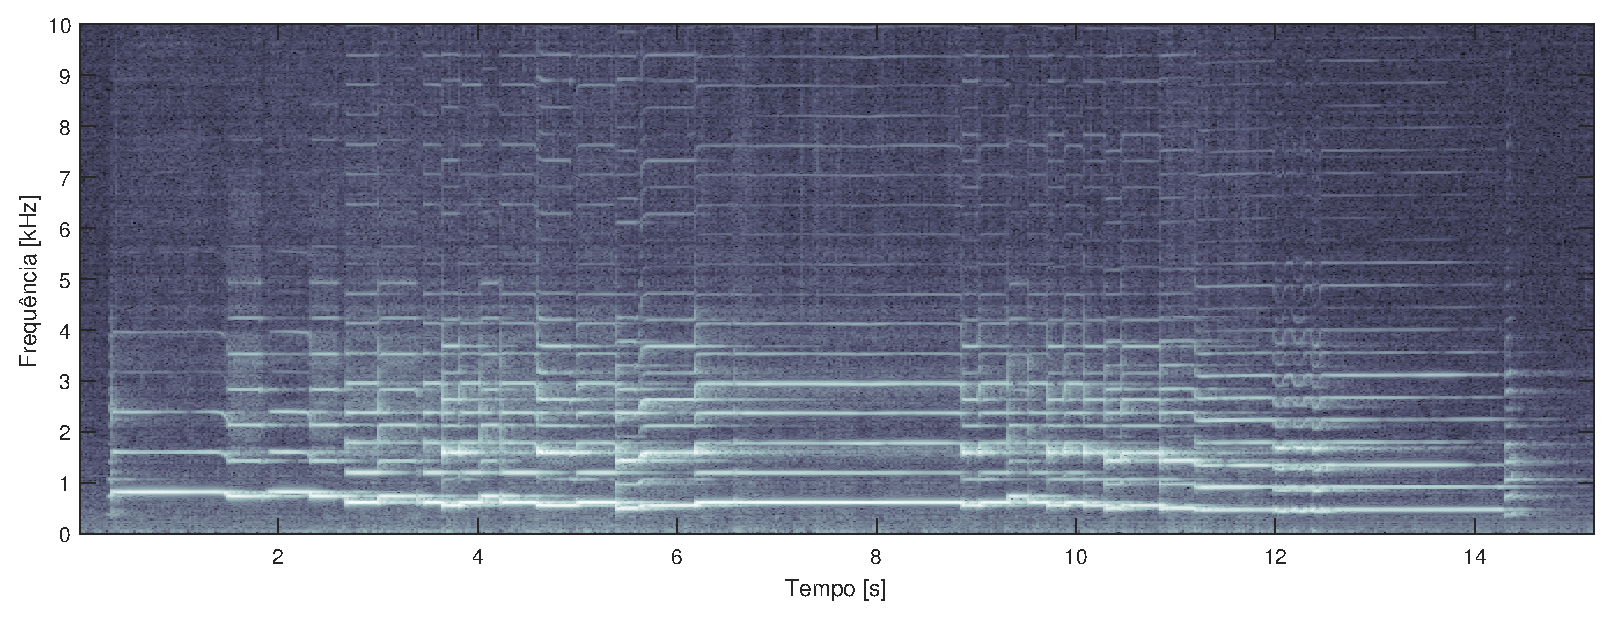
\includegraphics[width=\linewidth]{wiener/wiener-reference-signal.eps}
	\caption[Espetrograma do sinal original usado nos experimentos]{Espectrograma do sinal original utilizado nos experimentos.}
	\label{fig:wf:spectogram-reference}
\end{figure}
\begin{figure}[!ht]
	\centering
	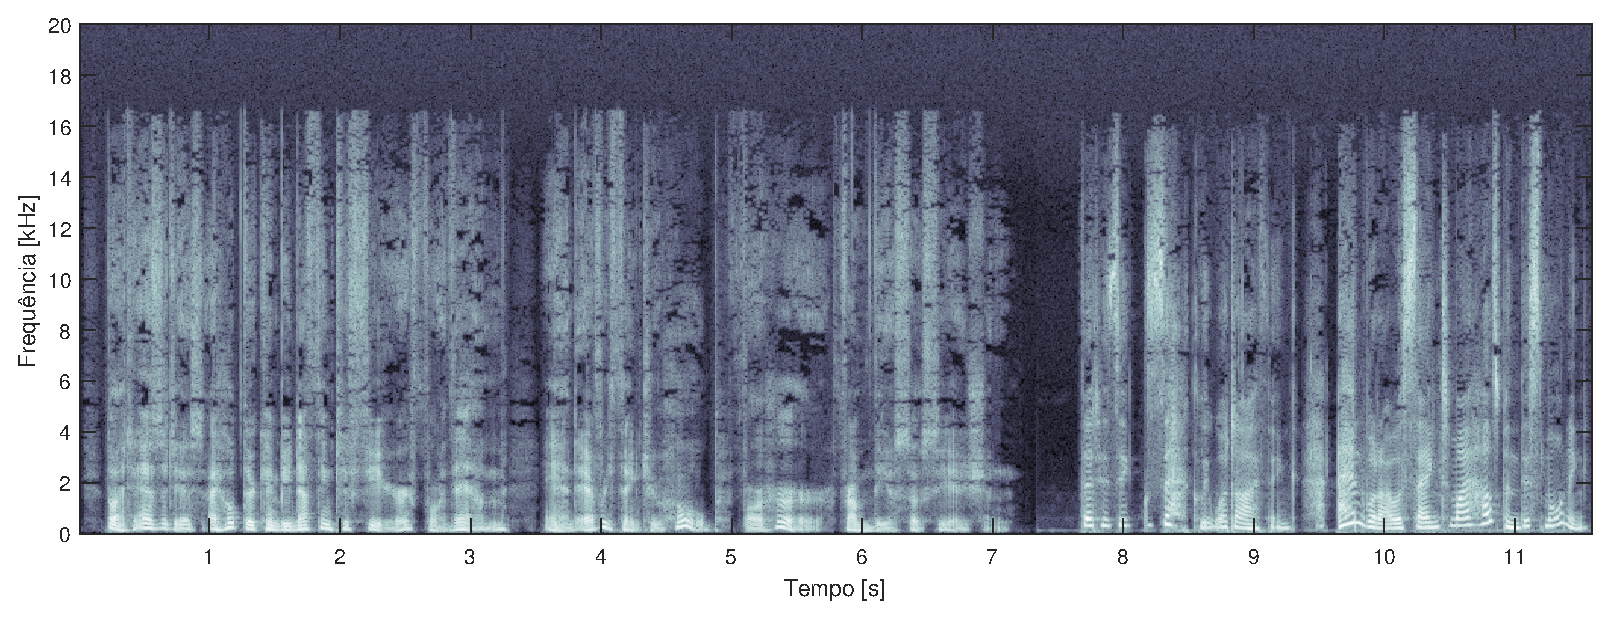
\includegraphics[width=\linewidth]{wiener/wiener-dialogue-signal.eps}
	\caption[Espetrograma do ruído usado nos experimentos]{Espectrograma da gravação de diálogo (a ser interpretada como ruído) utilizada nos experimentos.}
	\label{fig:wf:spectogram-dialogue}
\end{figure}

Em relação à janela escolhida para o método de \textit{overlap-add}, foi priorizado um
janelamento que aplicasse ganho unitário ao sinal sintetizado, para que não fosse
necessário um pós-processamento de correção de ganho. Nas devidas condições, a função
de Hann de comprimento $M$ definida como
\begin{equation}
	h^2[n] = \frac{1}{2} - \frac{1}{2}\cos\left(\frac{2\pi n}{M}\right) = \sen^2\left( \frac{\pi n}{M} \right),\ 0 \leq n \leq M-1,
\end{equation}
cumpre esse requisito: com $M$ par, uma sobreposição de $50\%$ ($H = M/2$) resulta em \textit{overlap-add} constante com ganho unitário~\cite{heinzel-2002}. Por este motivo, a janela estipulada foi escolhida com base na função de Hann. Porém, como explicitado na seção anterior, o janelamento será aplicado duas vezes ao sinal, e, portanto, precisamos de que sua versão quadrática satisfaça a condição de COLA. Assim, a janela $h[n]$ que foi usada é a raiz quadrada da descrita anteriormente:
\begin{equation}
	h[n] = \sqrt{\frac{1}{2} - \frac{1}{2}\cos\left(\frac{2\pi n}{M}\right)} = \sen\left( \frac{\pi n}{M} \right),\ 0 \leq n \leq  M-1.
\end{equation}

Todos os experimentos foram executados com filtros de tamanho $L = 34$, janelas de
comprimento $M = 2^{13} = 8192$ (aproximadamente $186$ ms), e, consequentemente, saltos
de $H = 4096$ amostras. Estes parâmetros foram definidos após múltiplos testes com
diferentes valores terem sido realizados. Tais escolhas apresentaram o melhor resultado
geral.

\subsection{\textit{Fades}}

Para o primeiro experimento, o sinal distorcido foi gerado aplicando-se um
\textit{fade-out} e um \textit{fade-in} no início e no final, respectivamente, da
gravação original. Para isso, foi utilizada a ferramenta de envoltória do Audacity, na
qual a transição entre ganhos é feita seguindo uma curva exponencial. Para o
\textit{fade-out}, os parâmetros do ganho foram $A_\mathrm{i} = 1$ e $A_\mathrm{f} =
	0.2$. Similarmente, no \textit{fade-in} estes parâmetros foram $A_\mathrm{i} = 0.2$ e
$A_\mathrm{f} = 1$. Ambos os efeitos duraram aproximadamente 1.5 segundo. O ruído não
foi adicionado à mixagem final. Assim, avaliamos a capacidade do método em estimar o
processamento de um sistema linear variante no tempo. Os resultados encontram-se na
Tabela~\ref{tab:wf:experiment-1}. {\def\arraystretch{1.25}\tabcolsep=10pt
\begin{table}[!ht]
	\centering
	\caption[Resultados do primeiro experimento: \textit{fades}]{Resultados do primeiro experimento.}
	\label{tab:wf:experiment-1}
	\begin{tabular}{cccc}
		\toprule
		               & SDR         & PAQM (MOS) & $\log_{10}(R_{\text{nonlin}})$ \\
		\midrule
		$(d, x)$       & $-11.57$ dB & $1.17$     & $-0.005$                       \\
		$(d, \hat{d})$ & $42.65$ dB  & $2.04$     & $-0.006$                       \\ \bottomrule
	\end{tabular}
\end{table}
}

Ao observarmos apenas os resultados da SDR, podemos concluir que o método estimou de
forma satisfatória a distorção que foi aplicada à gravação original. Por outro lado, se
considerarmos apenas a PAQM, a melhoria não parece ter sido tão satisfatória assim.
Porém, não podemos nos esquecer que a rigorosa compressão aplicada pela transformação
dos resultados de $\log_{10}(\mathcal{L}_n)$ em MOS pode resultar em valores baixos
mesmo em sinais muito similares. Assim, não podemos nos ater apenas ao valor absoluto
do resultado, e sim interpretá-lo no contexto geral; neste caso, a nota aproximadamente
dobrou de valor.

É interessante notar também a queda no valor de $\log_{10} (R_{\text{nonlin}})$ para $(d, \hat{d})$. Isto ocorreu pois o algoritmo empregado (com \textit{overlap-add}) não é estritamente linear; por exemplo, as últimas $L - 1$ amostras geradas na convolução de cada intervalo não são utilizadas no processo de estimação.\footnote{Se um sinal de comprimento $M$ é convoluído com um filtro de tamanho $L$, a saída resultante terá tamanho $M+L-1$. Porém, como a janela também tem tamanho $M$, foi necessário descartar as últimas $L-1$ amostras de cada iteração para realizarmos o \textit{overlap-add}.} Portanto, é possível que o método introduza não-linearidades indesejadas ao sinal de entrada. Mesmo assim, estas supostas distorções detectadas foram virtualmente inaudíveis.

\subsection{\textit{Fades} com ruído aditivo} \label{subsec:wiener:experiment-2}

No segundo experimento, foi considerada exatamente a mesma versão distorcida do teste
anterior. Porém, agora, à mixagem final foi somado o ruído; assim, o sinal distorcido
foi usado como trilha de fundo para o diálogo. Com isso, avalia-se a robustez do método
a sinais espúrios (com um caso extremo, já que o ruído está mais intenso que o sinal
desejado). A SNR da observação é $-9.17$~dB. Os resultados encontram-se na
Tabela~\ref{tab:wf:experiment-2}. {\def\arraystretch{1.25}\tabcolsep=10pt
\begin{table}[!ht]
	\centering
	\caption[Resultados do segundo experimento: \textit{fades} com ruído aditivo]{Resultados do segundo experimento.}
	\label{tab:wf:experiment-2}
	\begin{tabular}{cccc}
		\toprule
		               & SDR         & PAQM (MOS) & $\log_{10}(R_{\text{nonlin}})$ \\
		\midrule
		$(d, x)$       & $-11.57$ dB & $1.17$     & $-0.005$                       \\
		$(d, \hat{d})$ & $15.39$ dB  & $1.20$     & $-0.028$                       \\ \bottomrule
	\end{tabular}
\end{table}
}

Embora o algoritmo tenha melhorado as medidas, os valores pioraram quando comparados
aos do experimento anterior. Isto era esperado, visto que a trilha descorrelacionada
possuía maior energia na mixagem final. Deste modo, o método não conseguiu reproduzir
igualmente bem o processamento aplicado ao sinal original, resultando principalmente em
resquícios de ruído --- zumbidos ``metálicos'' --- nos instantes de maior intensidade
no diálogo.

\subsection{\textit{Soft clipping}}

No terceiro experimento, queremos avaliar a eficiência do método em replicar a
distorção não-linear de \textit{soft clipping}. No Audacity, a curva de limitação é uma
função definida por partes: linear entre $-0.5$ e $0.5$ e senoidal nas extremidades
(cada uma consiste em $1/8$ de um período de onda). A limitação é feita passando o
sinal por este mapeamento, que antes é normalizado para que seu valor máximo seja igual
ao pico de amplitude máximo especificado; no caso do experimento, este foi $-7.5$ dB. O
ruído não foi introduzido. Os resultados encontram-se na
Tabela~\ref{tab:wf:experiment-3}. {\def\arraystretch{1.25}\tabcolsep=10pt
\begin{table}[!ht]
	\centering
	\caption[Resultados do terceiro experimento: \textit{soft clipping}]{Resultados do terceiro experimento.}
	\label{tab:wf:experiment-3}
	\begin{tabular}{cccc}
		\toprule
		               & SDR        & PAQM (MOS) & $\log_{10}(R_{\text{nonlin}})$ \\
		\midrule
		$(d, x)$       & $19.56$ dB & $1.21$     & $-0.016$                       \\
		$(d, \hat{d})$ & $23.24$ dB & $1.22$     & $-0.016$                       \\ \bottomrule
	\end{tabular}
\end{table}
}

Podemos observar uma pequena melhora nos valores da SDR e da PAQM, e nenhuma alteração
no valor do $\log_{10}(R_{\text{nonlin}})$. Temos aqui o primeiro exemplo das
limitações do Filtro de Wiener, que não consegue reproduzir a distorção não-linear
aplicada ao sinal original; o incremento provavelmente se deu porque o algoritmo é
capaz de aplicar uma atenuação aos picos, mas não um ceifamento.

\subsection{\textit{Soft clipping} com ruído aditivo}

Neste experimento, somamos a trilha de diálogo ao sinal fabricado no experimento
anterior. É importante notar que não foi aplicado nenhum outro processamento ao sinal
distorcido, portanto, a SNR está maior do que a encontrada no
Experimento~\ref{subsec:wiener:experiment-2}, sendo $3.97$~dB. Os resultados
encontram-se na Tabela~\ref{tab:wf:experiment-4}.
{\def\arraystretch{1.25}\tabcolsep=10pt
\begin{table}[!ht]
	\centering
	\caption[Resultados do quarto experimento: \textit{soft clipping} com ruído aditivo]{Resultados do quarto experimento.}
	\label{tab:wf:experiment-4}
	\begin{tabular}{cccc}
		\toprule
		               & SDR        & PAQM (MOS) & $\log_{10}(R_{\text{nonlin}})$ \\
		\midrule
		$(d, x)$       & $19.56$ dB & $1.21$     & $-0.016$                       \\
		$(d, \hat{d})$ & $22.11$ dB & $1.20$     & $-0.022$                       \\ \bottomrule
	\end{tabular}
\end{table}
}

Observe que, mesmo com a melhoria no valor da SDR, houve uma piora nos valores das
outras duas medidas. Ao ouvir a estimação resultante, o porquê disso se torna evidente:
novamente temos resquícios do diálogo em alguns instantes do sinal estimado, mas, além
disso, possivelmente também artefatos do algoritmo, visto que, como demonstrado melhor
no próximo experimento, o método é capaz de introduzir ruídos no sinal distorcido.

\subsection{\textit{Fades} e codificação com perdas} \label{subsec:wiener:experiment-5}

Como o processo de codificação costuma ser executado ao fim de uma mixagem, após outras
distorções terem sido aplicadas, iremos utilizar o sinal distorcido do primeiro
experimento como entrada no algoritmo de codificação. A gravação de diálogo não foi
adicionada. Foi aplicada uma codificação MP3 com taxa de bits constante de 56 kbps
usando a biblioteca LAME\abbrev{LAME}{LAME \textit{Ain't an} MP3
	\textit{Encoder}}~\cite{lame-encoder}. Os resultados encontram-se na
Tabela~\ref{tab:wf:experiment-5}. {\def\arraystretch{1.25}\tabcolsep=10pt
\begin{table}[!ht]
	\centering
	\caption[Resultados do quinto experimento: \textit{fades} e codificação com perdas]{Resultados do quinto experimento.}
	\label{tab:wf:experiment-5}
	\begin{tabular}{cccc}
		\toprule
		               & SDR         & PAQM (MOS) & $\log_{10}(R_{\text{nonlin}})$ \\
		\midrule
		$(d, x)$       & $-14.77$ dB & $1.17$     & $-0.032$                       \\
		$(d, \hat{d})$ & $13.43$ dB  & $1.18$     & $-0.080$                       \\ \bottomrule
	\end{tabular}
\end{table}
}

É possível notar que, embora a SDR tenha ficado com um valor próximo ao do segundo experimento, a PAQM e o $\log_{10}(R_{\text{nonlin}})$ denunciam a baixa similaridade psicoacústica entre o sinal distorcido e o estimado (quando comparados aos outros resultados). Ademais, ao tentar reproduzir distorções não-lineares usando um sistema linear, o algoritmo introduziu artefatos na estimação, o que explica a queda significativa no valor de $\log_{10}(R_{\text{nonlin}})$.

\subsection{\textit{Fades} com ruído aditivo e codificação com perdas} \label{subsec:wiener:experiment-6}

Para este último teste, codificou-se o áudio gerado no segundo experimento: o sinal
$x[n]$ com \textit{fades} e diálogo somado. Os parâmetros da codificação foram os
mesmos do quinto experimento. É importante mencionar que, neste caso, não é possível
obter a versão isolada exata do sinal distorcido na observação, já que o processo de
codificação, por ser não-linear, utiliza uma combinação não-trivial entre a entrada e o
ruído. Por este motivo, como $d[n]$ usaremos o mesmo sinal distorcido gerado no
Experimento~\ref{subsec:wiener:experiment-5}, que pressupomos ser
\emph{aproximadamente} igual ao valor da versão do sinal presente em $y[n]$. Não foi
possível calcular a SNR dessa observação, mas podemos estimar seu limite superior como
sendo $-9.17$~dB. Os resultados encontram-se na Tabela~\ref{tab:wf:experiment-6}.
{\def\arraystretch{1.25}\tabcolsep=10pt
\begin{table}[!ht]
	\centering
	\caption[Resultados do sexto experimento: \textit{fades} com ruído aditivo e codificação com perdas]{Resultados do sexto experimento.}
	\label{tab:wf:experiment-6}
	\begin{tabular}{cccc}
		\toprule
		               & SDR         & PAQM (MOS) & $\log_{10}(R_{\text{nonlin}})$ \\
		\midrule
		$(d, x)$       & $-14.77$ dB & $1.17$     & $-0.032$                       \\
		$(d, \hat{d})$ & $11.47$ dB  & $1.18$     & $-0.087$                       \\ \bottomrule
	\end{tabular}
\end{table}
}

Os resultados são a culminação de tudo que vimos até agora nos experimentos. Se, por um
lado, o modelo consegue estimar a variação de amplitude, por outro, o processamento
não-linear --- junto à baixa razão sinal-ruído --- dificulta a estimação, sendo isso
refletido principalmente no quesito psicoacústico.
